%%%%%%%%%%%%%%%%%%%%%%%%%%%%%%%%%%%%%%%%%
% Journal Article
% LaTeX Template
% Version 1.3 (9/9/13)
%
% This template has been downloaded from:
% http://www.LaTeXTemplates.com
%
% Original author:
% Frits Wenneker (http://www.howtotex.com)
%
% License:
% CC BY-NC-SA 3.0 (http://creativecommons.org/licenses/by-nc-sa/3.0/)
%
%%%%%%%%%%%%%%%%%%%%%%%%%%%%%%%%%%%%%%%%%

%----------------------------------------------------------------------------------------
%	PACKAGES AND OTHER DOCUMENT CONFIGURATIONS
%----------------------------------------------------------------------------------------

\documentclass[twoside]{article}

\usepackage{lipsum} % Package to generate dummy text throughout this template

\usepackage[sc]{mathpazo} % Use the Palatino font
\usepackage[T1]{fontenc} % Use 8-bit encoding that has 256 glyphs
\linespread{1.05} % Line spacing - Palatino needs more space between lines
\usepackage{microtype} % Slightly tweak font spacing for aesthetics
\usepackage{graphicx}
\usepackage[hmarginratio=1:1,top=32mm,columnsep=20pt]{geometry} % Document margins
\usepackage{multicol} % Used for the two-column layout of the document
\usepackage[hang, small,labelfont=bf,up,textfont=it,up]{caption} % Custom captions under/above floats in tables or figures
\usepackage{booktabs} % Horizontal rules in tables
\usepackage{float} % Required for tables and figures in the multi-column environment - they need to be placed in specific locations with the [H] (e.g. \begin{table}[H])
\usepackage{hyperref} % For hyperlinks in the PDF
\usepackage{subcaption}

\usepackage{lettrine} % The lettrine is the first enlarged letter at the beginning of the text
\usepackage{paralist} % Used for the compactitem environment which makes bullet points with less space between them

\usepackage{abstract} % Allows abstract customization
\renewcommand{\abstractnamefont}{\normalfont\bfseries} % Set the "Abstract" text to bold
\renewcommand{\abstracttextfont}{\normalfont\small\itshape} % Set the abstract itself to small italic text

\usepackage{titlesec} % Allows customization of titles
\renewcommand\thesection{\Roman{section}} % Roman numerals for the sections
\renewcommand\thesubsection{\Roman{subsection}} % Roman numerals for subsections
\titleformat{\section}[block]{\large\scshape\centering}{\thesection.}{1em}{} % Change the look of the section titles
\titleformat{\subsection}[block]{\large}{\thesubsection.}{1em}{} % Change the look of the section titles

\usepackage{fancyhdr} % Headers and footers
\pagestyle{fancy} % All pages have headers and footers
\fancyhead{} % Blank out the default header
\fancyfoot{} % Blank out the default footer
\fancyhead[C]{} % Custom header text
\fancyfoot[RO,LE]{\thepage} % Custom footer text

%----------------------------------------------------------------------------------------
%	TITLE SECTION
%----------------------------------------------------------------------------------------

\title{\vspace{-15mm}\fontsize{24pt}{10pt}\selectfont\textbf{League of Legends: Preliminary Data Analysis}} % Article title

\author{
\large
\textsc{Alyssa M. Adams}\thanks{Expert Teemo player (Gold I)}\\[2mm] % Your name
\normalsize Arizona State University, Tempe \\ % Your institution
\normalsize \href{mailto:alyssa.gp.adams@gmail.com}{alyssa.gp.adams@gmail.com} % Your email address
\vspace{-5mm}
}
\date{}

%----------------------------------------------------------------------------------------

\begin{document}

\maketitle % Insert title

\thispagestyle{fancy} % All pages have headers and footers

%----------------------------------------------------------------------------------------
%	ABSTRACT
%----------------------------------------------------------------------------------------

\begin{abstract}

\noindent The online video game League of Legends has a massive, easy-to-access dataset that can be used to analyze in terms of information theory. This paper reports on the progress of the project LoLIntelligence, which is a Python package that analyzes the dataset to understand the dynamics between players and game developers. These dynamics play as a form of distributed computation that performs open-ended evolution in a system, which is a well-known feature of biological systems. A small subset of the data was used to develop information-theoretic measures across the data as a function of time. It was found that a small subset of game champions store and process high amount of information consistently over time. This suggests the network of player-developer interactions heavily relies on a small subset of champion statistics, which suggests the network can be analyzed in terms of controlability.
\end{abstract}

%----------------------------------------------------------------------------------------
%	ARTICLE CONTENTS
%----------------------------------------------------------------------------------------

\begin{multicols}{2} % Two-column layout throughout the main article text

\section{Introduction}

\lettrine[nindent=0em,lines=3]{L}eague of Legends (LoL) is an online team-based strategy game that has become immensely popular over the last six years and is currently the most popular game of its type (1). Riot, the game's developer, has made data generated by the game free to the public. This data includes a complete set of statistics for every individual game instance played across the world during the last four years. Independent websites developed applications that process this data in a variety of way, such any player's match history (lolking.com), approximate MMR (op.gg), and how much time a player has spent on LoL (wasted-on-lol.com).

Even with the vast number of web applications that use LoL data, the data has yet to be studied by scientists in most fields. Social systems, like League of Legends, have been notoriously difficult to study because they are complex systems, which have yet to be defined mathematically (2). One of the factors that contributes to the lack of understanding is lack of good data. Since LoL has a fairly complete dataset, it is an excellent platform for studying complex social systems.

This paper reports on a first attempt to analyze this data in an \textit{information-theoretic sense}. Since the data is so vast, only a very small subset is used to develop methods of measurement and analysis. I use my own match history as I main Teemo over a time period of two weeks. In the future, a much larger dataset of challenger/master players will be analyzed in the same way. 



\section{Some Assumptions}

\paragraph{Strategy} Typically, a player's combination of champion and position indicates the playstyle they wish to engage in the game, and is hence dubbed a player's \textit{strategy}. As an example, if a player picks the champion Teemo and the position Support, then both teams expect the player to play Teemo using a particular strategy throughout the game. The combination of all five team players' strategies combine into a \textit{team strategy}. In general, the frequency of types of individual and team strategies change over time based on what strategies are popular in the game community as a whole.

\paragraph{Ranked Games} Games that are ``ranked'' place players on a skill tier system based on how many games they have won. The Bronze tier houses the lowest skill players, while Challenger tier houses players that likely play on professional teams. Winning many games over time increases the chances a player will climb the tier. For a single game, I assume that players are randomly matched with players in the same tier, or close to. I also only look at data from ranked games, since I assume players will be using their best individual strategies for these games.



\section{League is like Biology} Over the last few years, I've been studying a system that has a type of ``environment'' that interacts with an ``organism'' (although no direct parallels between this system and an actual organism are made)\footnote{The formal preprint for this report is attached with this application.}. The organism is changed by signals within itself and also signals from the environment. As a result, the organism is much more complex than an organism that does not interact with an environment (3). League resembles this system in the sense that it has an ``environment'' (the game developers introducing changes) and an ``organism'' (player behaviors and strategies). 

The interaction between the environment and organism result in the organism being open-ended, which is something commonly observed in complex systems. Open-endedness generally refers to a system never repeating and constantly innovating, much like biological evolution. Up until recently, it has been a mystery in complex systems (3). Since we understand how open-endeness works in a simple model, we can use the same principles to understand how open-endedness is driven in LoL. \textbf{If we can understand this, then we can understand how the data changes over time as changes are introduced to the game.}

\paragraph{Internal Mechanisms} Without any interference from Riot, internal mechanisms from the players seem to resemble a negative frequency-dependent selection strategy.  This type of frequency-dependent selection is well-known in population dynamics of competing species (4). In LoL, this can be seen with rotating metas: when tanks become popular, anti-tanks gain popularity and tanks are no longer the meta. Over time, the counters to the anti-tanks become popular, and those anti-tanks are old news. In other words, the game is not static by any means and changes according to current player behaviors. 

These internal dynamics are driven by players, depending on what is the most popular or strong in the current meta. In addition, professional players' strategies influence the meta as well, with the most successful strategies as ones being used in the LCS or World Championship. Professional players set many trends that most other players work to imitate. Using Teemo as an example, one professional player started playing Teemo as a high-damage character in the Top position while other players were playing him in the Mid position. Since many people watch this player's behavior, many imitated this player's Teemo strategy which is a trend that continues today.

League of Legends is notorious for having a ``toxic'' player community, meaning many players can be unfriendly and bully each other around during games. Efforts are constantly enforced to minimize the effects of toxic players by the game developers, which has had some success (5). From a behavioral-ecological standpoint, it is easy to notice the structure of the game is deeply affected by player behavior. For example, toxic players cause many players to surrender games early, which affects the overall statistics of the game. In general, toxic players often lose much more than other players, thus placing them in lower tiers. This makes it extremely difficult for non-toxic to climb out of lower tiers, and any strategies seen in lower tiers are generally considered ``bad gameplay strategies''. Therefore, the majority player community avoids particular gameplay strategies because of their lower-tier association, changing the gameplay across all skill tiers.

\paragraph{External Mechanisms} External mechanisms introduced by Riot change the landscape of possible strategies. The frequency of patches or changes highly influences the internal dynamics of gameplay. Both internal and external mechanisms are what make LoL so much fun, since it keeps the game out of equilibrium.


%------------------------------------------------

\section{Creating a Network}
All the above can be represented as a network in several different ways, each highlighting an aspect of the game. On paper, there is no concept of one champion being better than another champion at any given time without players actually playing the game. As players play the game, the popularity of any given champion (where the champion becomes popular for a variety of reasons) creates a dynamic hierarchy of preferred champions. If the champion Teemo becomes very popular, many players will assume Teemo is a very good pick at the moment. However, this might not actually reflect the actual amount of games player who play Teemo actually win. A champion's \textbf{winrate} is the actual number of games players who play that given champion win overall.

\paragraph{Champion Counter-network}
At any given time, a network can be constructed to show which champion beats (\textit{counters}) which champion based on the win/loss outcomes of players who play those champions. According to counterstats.net (6), Teemo beats another champion named Renekton in the Mid position because Teemo has the higher winrate for that position. In other words, Teemo wins more often than Renekton in the Mid position so Teemo is considered to counter Renekton. 

This can be represented on a graph as Teemo and Renekton as nodes. A directed edge that goes from Teemo into Renekton indicates that Teemo counters Renekton. Winrate statistics can be found for every champion in every position. These statistics can be used to build a counter-network for every champion in League of Legends. This network is shown in Figure 5, where each node has a minimum of one in-degree and one out-degree. Labels for nodes are not shown.

\begin{figure*}
  \centering
    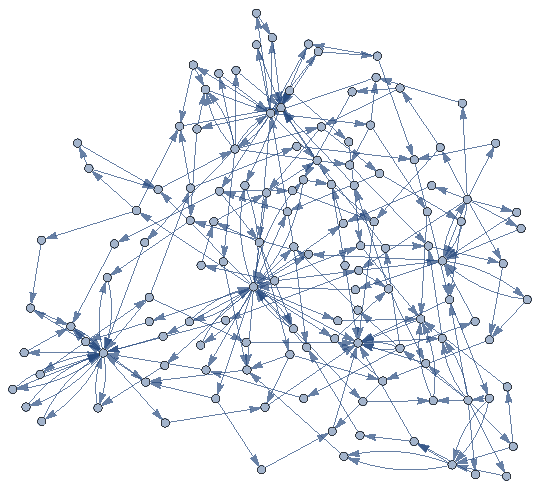
\includegraphics[width=0.5\textwidth]{metagraph.pdf}
  \caption{A network that shows how champions (nodes) beat (directed edges) other champions.}
  \label{fig:workflowedge}
\end{figure*}

An immediate question to ask is whether or not the vertex out-degree of a champion correlates with that champion's overall winrate. Figure 6 compares these two measures in color, where red indicates high values and blue indicates low values. Notice how the two measures seem to be much less correlated than intuition would lend. Champions that counter many other champions do not have the highest winrates.

\begin{figure*}
\centering
\begin{subfigure}{.5\textwidth}
  \centering
  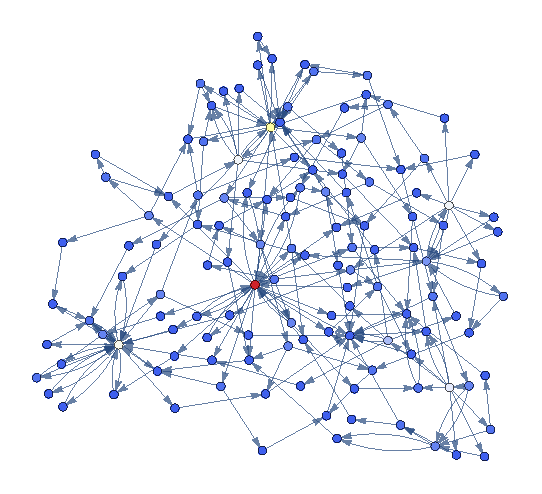
\includegraphics[width=1\linewidth]{outdegree.pdf}
  \caption{Node color indicates node out-degree, or the number of champions a given champion counters in game.}
  \label{fig:sub1}
\end{subfigure}%
\begin{subfigure}{.5\textwidth}
  \centering
  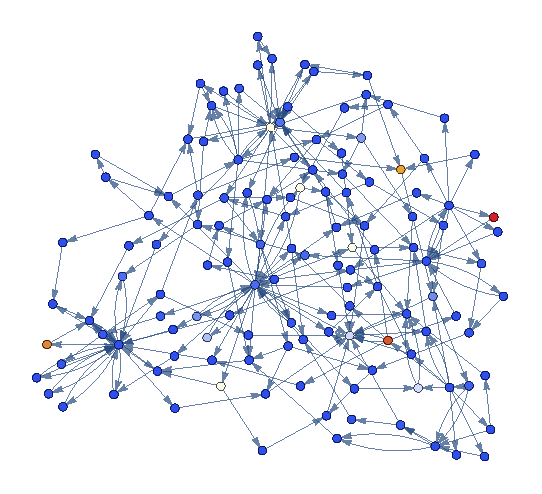
\includegraphics[width=1\linewidth]{prepop.pdf}
  \caption{Node color indicates the corresponding node's (champion's) winrate.}
  \label{fig:sub2}
\end{subfigure}
\caption{The same network in Figure 5 is shown with nodes colored given to out-degree (a) and winrate (b). Blue color indicates low values, while red color indicated high values. White colors indicate values that are in-between high and low.}
\label{fig:test}
\end{figure*}

\paragraph{Problem with Networks}
A problem immediately arises from the statistics that are used here. The winrates are heavily slanted by champion popularity and are not normalized. For example, the reason a particular node may have a high number of out-degrees is because that champion is simply popular and played in many different positions. Nodes that have only one in-degree and one out-degree might be unpopular champions for a large variety of reasons (the champion may be old and out-of-date graphically and is less aesthetically appealing).

An even bigger issue is that these networks change over time from the internal mechanisms discussed previously. On top of that, every few months a new node is introduced to the network when the developers add a new champion to the game. Champions are never removed from the game. In addition, old champions are changed or updated or spatial properties of the map are physically altered. All these changes affect this network drastically and as a result, edges are re-wired on a daily basis. 

\paragraph{Collecting better data}
In order to avoid the most extreme network changes, any further data used for analysis will only be used from times where the game developers did not make changes to the game. Any changes to the network result from internal player feedback mechanisms. 

To further reduce the data set, I only consider a 50-game match history segment from my own games. Data is collected directly from the game developers through a set of Python 3.0 scripts known as Casseopiea (7). These games span over the course of 14 days. This automatically introduces a strong bias towards the playstyle of a single player, but the idea is to develop scalable measures to eventually analyze much larger ensembles of games for many different players. With more data, general statements about the game as a whole can be made.

In order to better understand the subset of data that is used throughout the rest of this paper, the champion counter-network for these 50 games is shown in Figure 7. Note how the center node has the highest in-degree and out-degree. This is a reflection of the bias introduced by the small amount of data from a single player used for this analysis.

\begin{figure*}
  \centering
    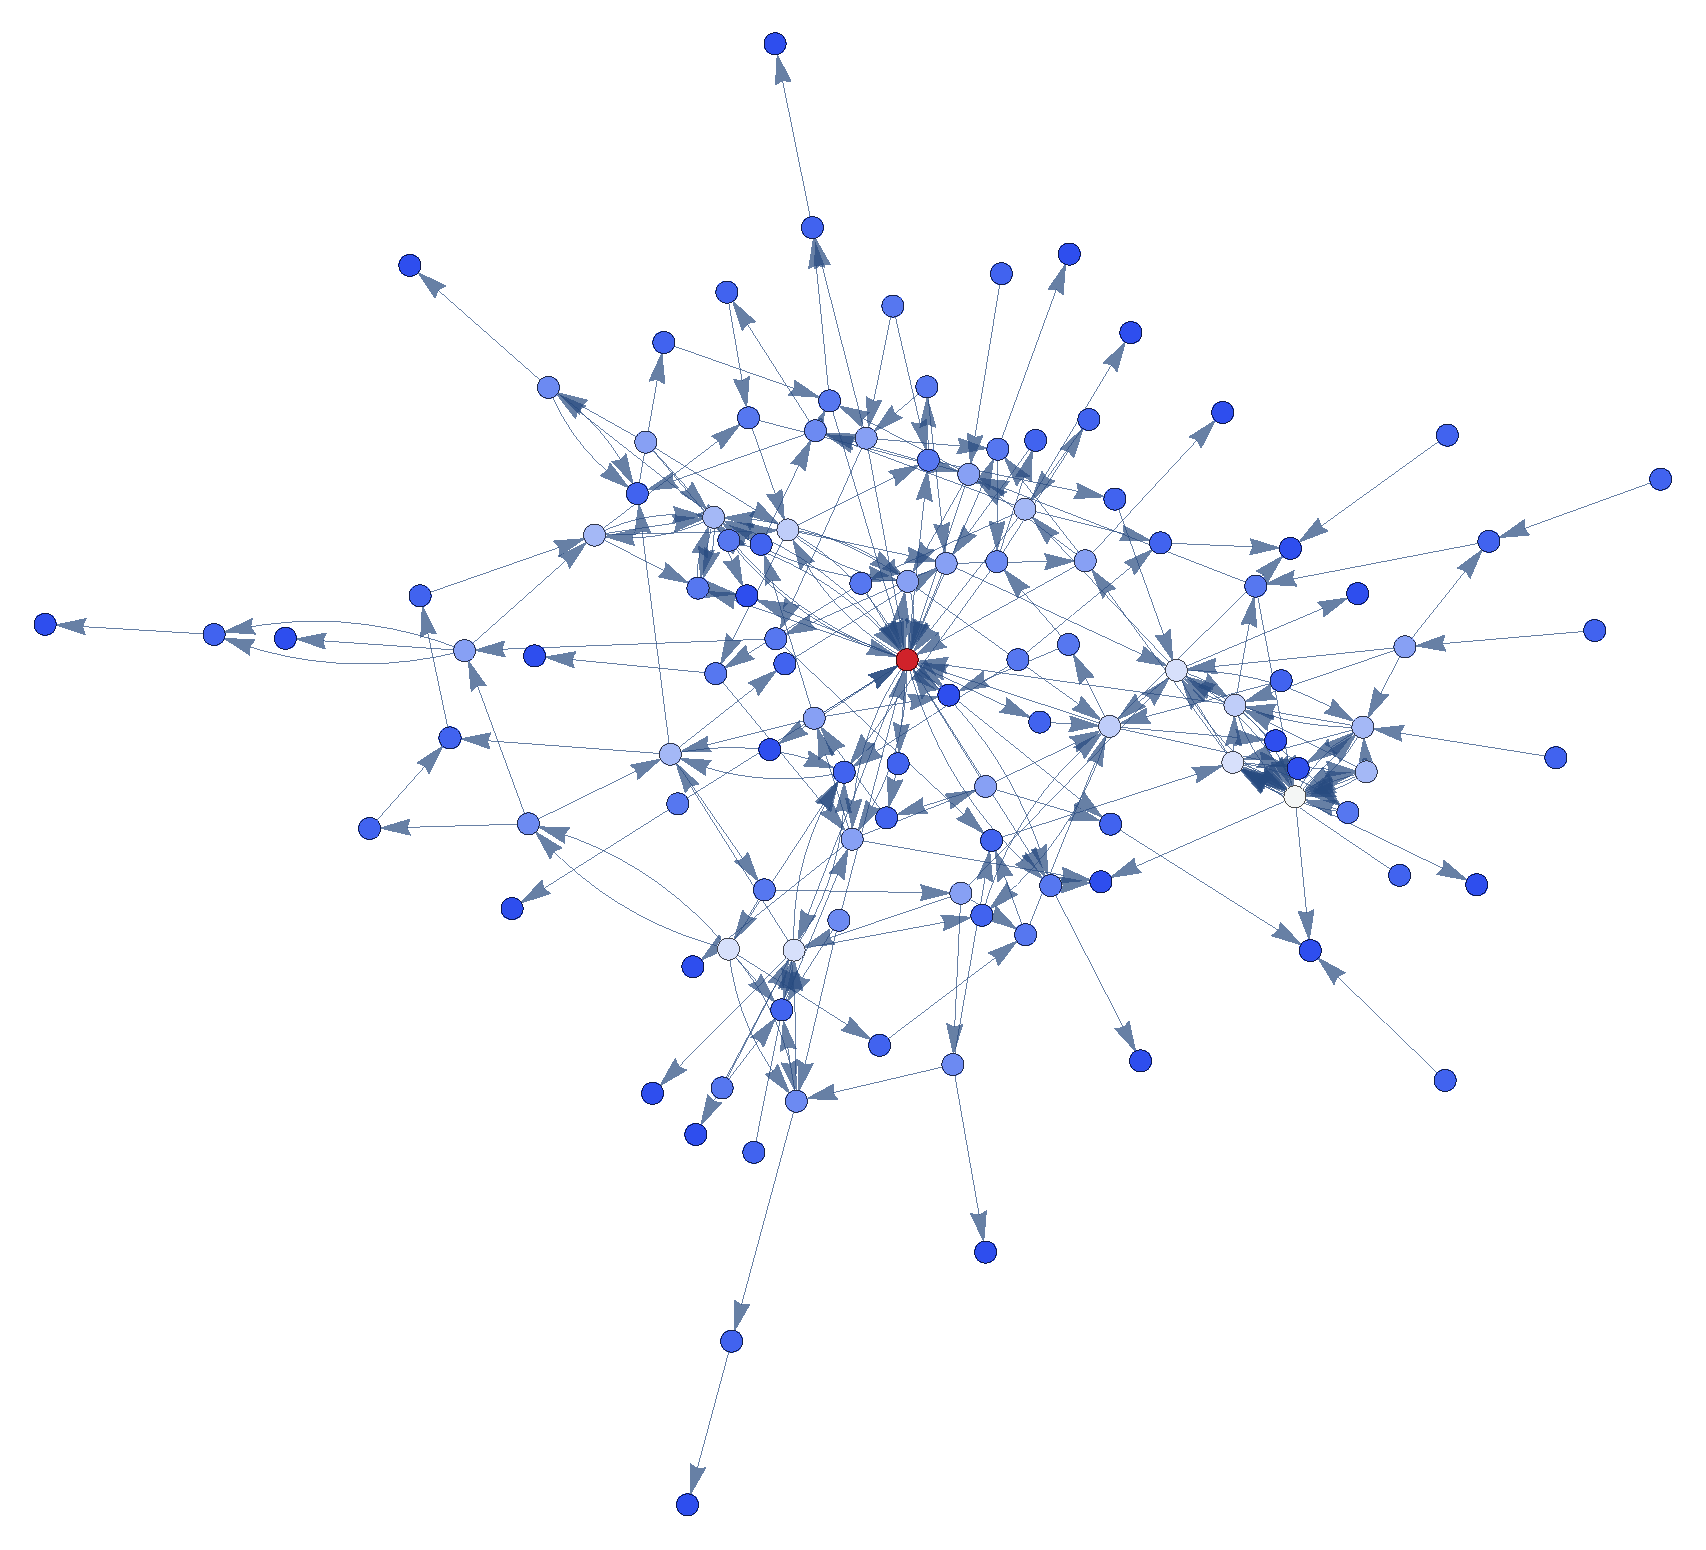
\includegraphics[width=0.6\textwidth]{teemocounternetwork.pdf}
  \caption{A network that shows how champions (nodes) beat (directed edges) other champions for the 50-game period from my own match history. Nodes colors indicate the out-degree for the corresponding node. Blue color indicates low values, while red color indicated high values. White colors indicate values that are in-between high and low. Node how the central node has the highest out-degree value. This is the main champion (Teemo) played by the author and highlights the data biases for this analysis.}
  \label{fig:workflowedge}
\end{figure*}

Instead of analyzing the network as a typical network (since update rules are not defined to determine how node values, whatever values those may be, update from one timestep to the next), data will only be analyzed as a time series, regardless of the structure of the underlying network. It is assumed that the network changes on a daily basis so fully understanding how the network evolves is not yet possible. Keeping these things in mind, the analysis on the data based on information measures will be not depend on the network structure of dynamics, and instead based on Boolean values of nodes as they change over time (regardless of edges).

%------------------------------------------------

\section{Information Measures}
Active information and transfer entropy are Shannon-based ways of measuring information storage and processing (respectively) in a system (8). They do not require more than a time series of discrete values to calculate, which is a convenient measure to use with this particular data set, since it does not depend on any network dynamics.

\paragraph{Active information}In particular, active information is defined as the ability for a particular node to store information. Over discrete time steps, a node $x$ will have discrete values. For any given time $n$, active information is calculated by summing over all possible time steps the odds of finding a particular pattern of size $k$:

\begin{equation}
AI_x = \sum_{n} \log_{2} \frac{p(x_{n+1}, x_{n}^{k})}{p(x_{n+1})p(x_{n}^{k})}
\end{equation}

The size of $k$ is analogous to the history length, or memory, or a system. The more often a given pattern of size $k$ given a value at time $n$ is found over the time series in a given node, the higher the active information that node has. For nodes with Boolean values (only having a value of 0 or 1), the maximum active information a value can have is 1.

\paragraph{Transfer entropy}Almost similar to active information, transfer entropy calculates the likelihood that node $y$ will affect what node $x$'s value is given some history length of node $x$, $k$. For a single node, the transfer entropy is calculated for all possible interactions between other $y$ nodes:

\begin{equation}
TE_{y \rightarrow x} = \sum_{n} \log_{2} \frac{p(x_{n+1} | x_{n}^{k}, y_{n})}{p(x_{n+1} | x_{n}^{k})}
\end{equation}

The more often a given pattern of size $k$ given a value at time $n$ for $x$, \textit{while also considering} the value for another node $y$ is found over the time series in a given node, the higher the transfer entropy that node has. If a node has a high value (close to 1) for transfer entropy, then that node is easily affected by the states of other nodes and thus processes much information about the entire system.

\paragraph{Generating two time series}Since the subset of data being considered is so small, no complete networks (one where all champions are present) can be extracted. As a baseline to generate a time series, the data was sorted into days as a time unit. Two types of values for the time series were considered: champion winrate and champion popularity. The winrate was only considered between that champion and their opponent with the same position. In other words, even if Teemo's team lost the game, if Teemo beat his opponent in the middle position by earning more gold, then it is counted as a win for Teemo. If Teemo wins more games than he loses in a day, then the Teemo node is assigned a `winrate = 1' value for that day, otherwise the node is assigned a `winrate = 0'. Similarly, if Teemo was in more than a third of all games played that day, then that node is assigned a `popularity = 1', otherwise it gets a `popularity = 0'. These thresholds were arbitrarily chosen, and need further justification by investigation.

%------------------------------------------------

\section{Results}

To gain a general sense of the information dynamics in this data, both the AI and TE were calculated for both the popularity time series and the winrate time series (Figures 8 and 9, respectively). The values are ranked by frequency and different $k$ values are indicated by color. In general, AI increases with larger $k$ values, while TE decreases with larger $k$ values. AI values are much larger than TE values in both types of time series. Overall, this general information analysis reveals little difference between the two types of time series. 

Both of the observables in the network (winrate and popularity) show similar trends in the distribution of AI and TE value. This suggests that in the data used, both observables have the same affect on the game. Intuitively, one might think that a winrate data would have a higher impact on player behavior but these graphs suggest champion popularity has an equal effect. 

For both TE and AI, different champions occupy the highest values, but are fairly constant with different $k$ values. This may be a reflection of the small data size, but it could also indicate that certain champions may play a pivotal role in the network as a whole. For example, the champion Master Yi was in the digests regimes of AI for every $k$ value, which indicates this champion might play a pivotal role in the game dynamics as a whole. \textbf{Regardless of data bias, the fact that a small, single set of nodes populates the highest AI and TE values is an interesting feature of the game, and is worth exploring in further detail with a larger set of data.}

\begin{figure*}
\centering
\begin{subfigure}{.5\textwidth}
  \centering
  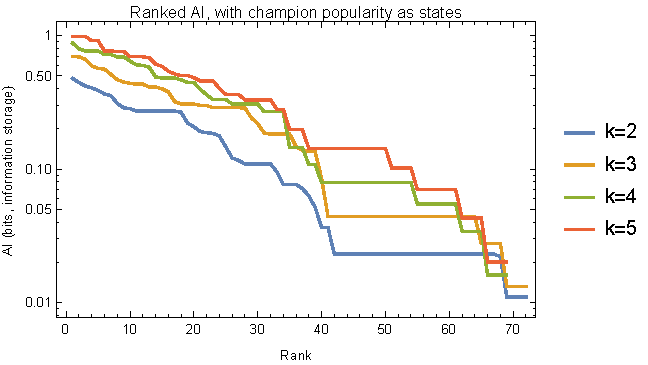
\includegraphics[width=1\linewidth]{population_AI_prelim.pdf}
  \caption{Popularity time series}
  \label{fig:sub1}
\end{subfigure}%
\begin{subfigure}{.5\textwidth}
  \centering
  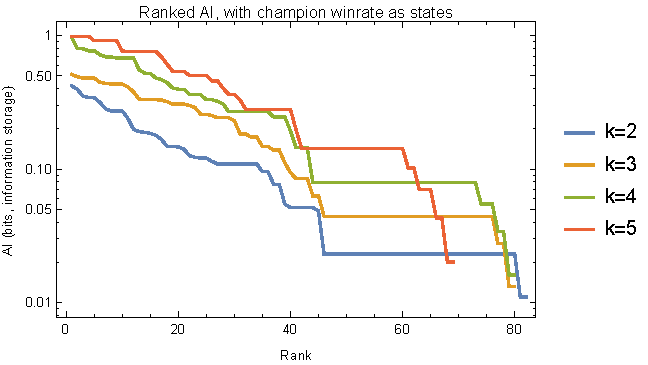
\includegraphics[width=1\linewidth]{winrate_AI_prelim.pdf}
  \caption{Winrate time series}
  \label{fig:sub2}
\end{subfigure}
\caption{The distribution of active information (AI) values are sorted by rank for both time series. Different colors indicate different values of k.}
\label{fig:test}
\end{figure*}

\begin{figure*}
\centering
\begin{subfigure}{.5\textwidth}
  \centering
  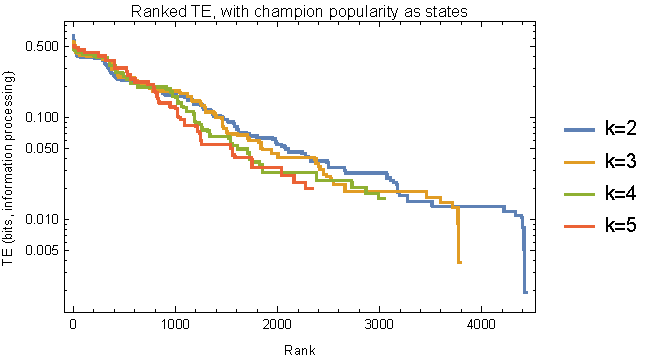
\includegraphics[width=1\linewidth]{popularity_TE_prelim.pdf}
  \caption{Popularity time series}
  \label{fig:sub1}
\end{subfigure}%
\begin{subfigure}{.5\textwidth}
  \centering
  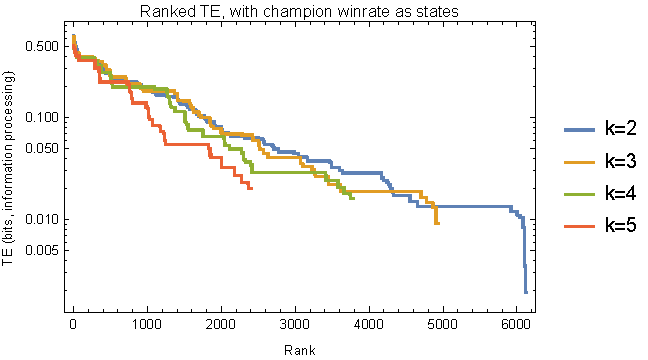
\includegraphics[width=1\linewidth]{winrate_TE_prelim.pdf}
  \caption{Winrate time series}
  \label{fig:sub2}
\end{subfigure}
\caption{The distribution of transfer entropy (TE) values are sorted by rank for both time series. Different colors indicate different values of k.}
\label{fig:test}
\end{figure*}

If TE is calculated only for nodes that are connected by an edge, the distribution of TE values changes a bit more between the two time series' (Figure 10). On average, TE values are slightly higher for winrate states. Most TE values are found between edges with a low average degree but in general, there is no clear trend between average vertex degree and TE. 

Again, the lack of a clear trend may be from small data bias. Figure 7 shows how the use of a single champion slants most of the player interactions to involve Teemo. Since one champion is unproportionally represented in this dataset, it probably has an affect on Figure 10.

\begin{figure*}
\centering
\begin{subfigure}{.5\textwidth}
  \centering
  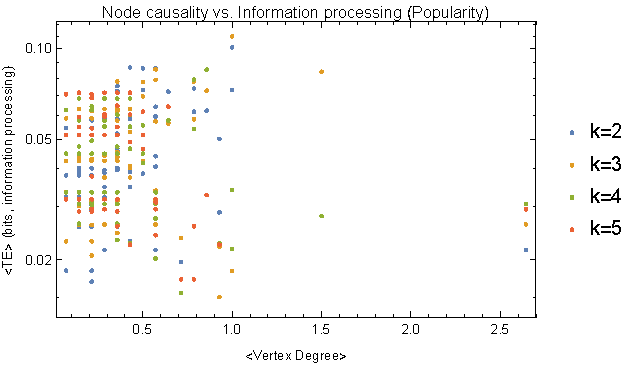
\includegraphics[width=1\linewidth]{popularity_degvsTE_prelim.pdf}
  \caption{Popularity time series}
  \label{fig:sub1}
\end{subfigure}%
\begin{subfigure}{.5\textwidth}
  \centering
  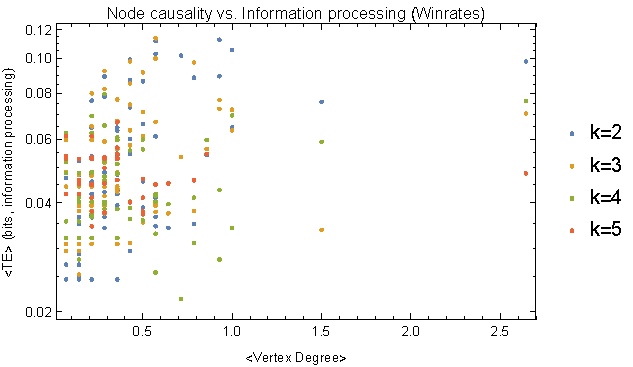
\includegraphics[width=1\linewidth]{winrate_degvsTE_prelim.pdf}
  \caption{Winrate time series}
  \label{fig:sub2}
\end{subfigure}
\caption{Average node degree (since node connectivity changes over time) vs. that node's average transfer entropy value. This is over the popularity time series. As before, different values for k are shown by color.}
\label{fig:test}
\end{figure*}

Because the data in Figure 10 lacks a clear trend, it is more informative to plot the total TE processed in each dataset as a function of $k$. Figure 11 shows a clear trend, and as seen in Figure 9, the total amount of information processed over a time series decreases as $k$ increases. The effect is more dramatic in the winrate time series, which suggests \textbf{information on what champion is winning has more causal power over smaller timescales than longer timescales, while information on champion popularity has more causal power over longer timescales than information on champion winrates}. Again, this is a trend worth exploring with a larger set of data to see if the same holds true for the game as a whole.

\begin{figure*}
\centering
\begin{subfigure}{.5\textwidth}
  \centering
  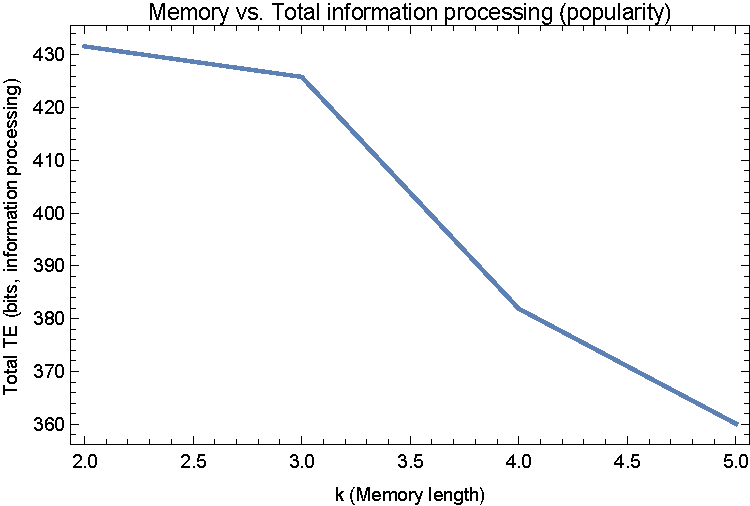
\includegraphics[width=0.9\linewidth]{popularity_memvsTE_prelim.pdf}
  \caption{Popularity time series}
  \label{fig:sub1}
\end{subfigure}%
\begin{subfigure}{.5\textwidth}
  \centering
  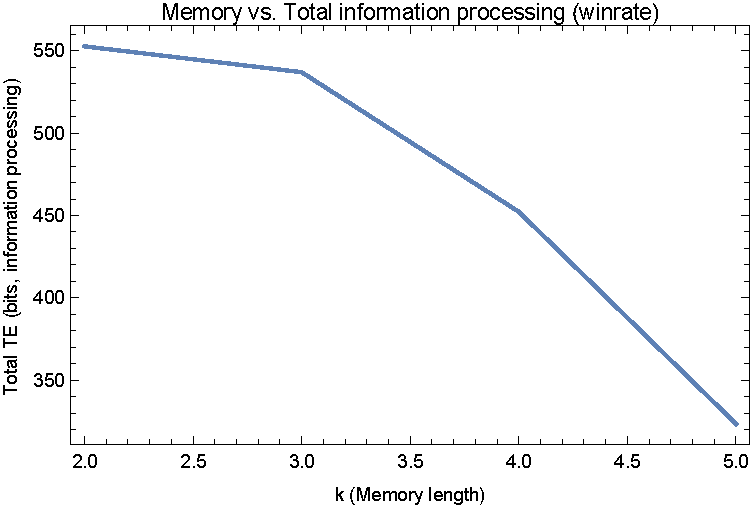
\includegraphics[width=0.9\linewidth]{winrate_memvsTE_prelim.pdf}
  \caption{Winrate time series}
  \label{fig:sub2}
\end{subfigure}
\caption{Total TE as a function of $k$ for both time series.}
\label{fig:test}
\end{figure*}

Finally, it will be useful to see the trend between AI and TE. Figures 12 and 13 show a heatmap of TE values as a function of AI. Nodes are arranged on the $x$ and $y$ axes according to their AI value. Nodes with low AI are towards the origin, while nodes with high AI are away from the origin. Both the $x$ and $y$ axis have the same arrangement for nodes. The distribution of the nodes' AI values is shown below the heatmap and it only shown for the $x$ axis since it is the same in the y axis. 

TE values are not symmetric, so the heatmap is not symmetric. The TE for a node A using B is different than node B using A. Each Figure shows data for a different $k$ value. These figures only represent data from the winrate time series, since the same figures produced by the popularity time series were not drastically different.

For low values of $k$, nodes with low AI values have, in general, higher TE values but as $k$ increases, this trend becomes more distributed over various AI values. Probably, this indicates that for this dataset, there is a core set of interactions that are the most meaningful in terms of causal power. Since the small data that is sampled involves many interactions with the same champion, many nodes were not included and results in many 0 values for TE and AI. However, \textbf{this relationship between TE and AI suggests a core number of champions have pivotal roles in the game dynamics}, as already suggested by Figure 8 (since the highest values for TE and AI are populated by a small subset of champions).

\begin{figure*}
\centering
\begin{subfigure}{.5\textwidth}
  \centering
  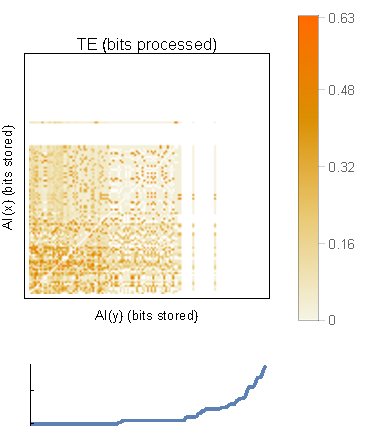
\includegraphics[width=0.9\linewidth]{winrate_AI_vs_AI_vs_TE_Heatmap_k2.pdf}
  \caption{$k=2$}
  \label{fig:sub1}
\end{subfigure}%
\begin{subfigure}{.5\textwidth}
  \centering
  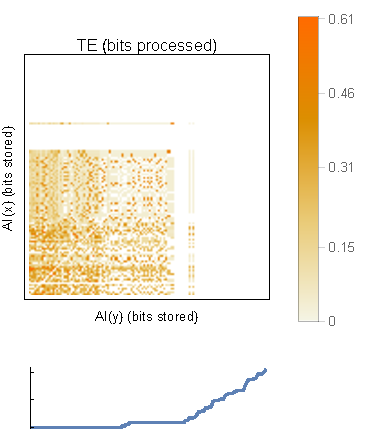
\includegraphics[width=0.9\linewidth]{winrate_AI_vs_AI_vs_TE_Heatmap_k3.pdf}
  \caption{$k=3$}
  \label{fig:sub2}
\end{subfigure}
\caption{Heatmap of TE values between nodes from the winrate time series. Nodes are arranged on the x and y axes according to their AI value. Nodes with low AI are towards the origin, while nodes with high AI are away from the origin. Both the x and y axis have the same arrangement for nodes. The distribution of the nodes' AI values is shown below the heatmap and it only shown for the x axis since it is the same in the y axis.}
\label{fig:test}
\end{figure*}

\begin{figure*}
\centering
\begin{subfigure}{.5\textwidth}
  \centering
  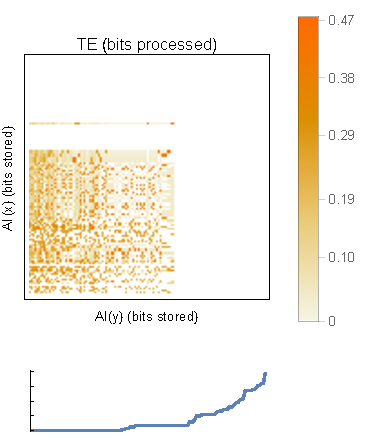
\includegraphics[width=0.9\linewidth]{winrate_AI_vs_AI_vs_TE_Heatmap_k4.pdf}
  \caption{$k=4$}
  \label{fig:sub1}
\end{subfigure}%
\begin{subfigure}{.5\textwidth}
  \centering
  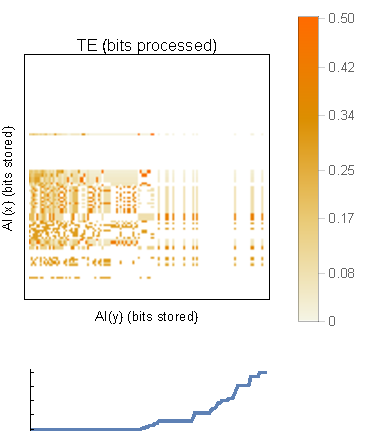
\includegraphics[width=0.9\linewidth]{winrate_AI_vs_AI_vs_TE_Heatmap_k5.pdf}
  \caption{$k=5$}
  \label{fig:sub2}
\end{subfigure}
\caption{Heatmap of TE values between nodes from the winrate time series. Nodes are arranged on the x and y axes according to their AI value. Nodes with low AI are towards the origin, while nodes with high AI are away from the origin. Both the x and y axis have the same arrangement for nodes. The distribution of the nodes' AI values is shown below the heatmap and it only shown for the x axis since it is the same in the y axis.}
\label{fig:test}
\end{figure*}

%------------------------------------------------

\section{Discussion}
The most striking results are shown by Figures 8 and 12. These figure indicate that most of the dynamics in the subset of games center around a small subset of champions. Interestingly, none of these ``central'' champions were Teemo, as intuition would suggest. Even though the dataset is small, this indicates a new notion of controllability. Since the same champions have high AI and TE values, they are perhaps controlling the overall game in some way. 

Figure 11 indicates that information processing occurs at a greater rate with a shorter memory in winrate dynamics than popularity dynamics. This might indicate that players process the most information about winrates in the last few days, but not over longer timescales. Over longer periods of time, champion popularity trends seem to have a bigger affect on the game in terms of information processing. This might be an indication of players' memory. Perhaps it is easier to remember which champions that were played, rather than which champions that have won.

Once again, all these results may be artifacts of a tiny sample size. The play habits of the single player are geared more towards playing Teemo over and over again, no matter the win or loss outcome. Regardless of this fact, the results are interesting, and it is worth investigating a larger dataset to see if these trends are a central feature of the game.

%------------------------------------------------

\section{What's Next?}
The algorithms developed for this analysis are certainly scalable with data size, so the most immediate step is to use data from a representative sample of the League of Legends community. Several questions are worth exploring to understand how this network behaves. Here are a few questions, ordered by tractability: 
\vspace{0.5cm}
\begin{compactitem}
\item How do these results change with different thresholds for winrate and popularity?
\item How do these results change with a representative sample of the entire League community? 
\item How do these results change from skill tier to skill tier? 
\item Is there a small subset of champions that ``control'' the game overall?
\item How do these results change as a function of player skill (sampling from each tier separately)?
\item How do these results change between patches per tier, specifically when a new node is added?
\item Are there nodes that have consistent AI and/or TE values?
\item What is the most sensitive part of the network, and does it change over time?
\end{compactitem} 
\vspace{0.5cm}
In addition, there are many questions that could result in direct applications: 
\vspace{0.5cm}
\begin{compactitem}
\item Are counter-networks intrinsic to champions or do they change with individual players?
\item If it is intrinsic to players, can this method be used to flag ``cheaters''?
\item How do intrinsic mechanisms signal Riot to make changes? Is there a consistent mapping between the two?
\end{compactitem} 
\vspace{0.5cm}
The goal is to understand how League of Legends behaves as an ecosystem of player behaviors, and to use this information to make predictions about the future. It seems like players perform a distributed computation to evolve the network, and then respond to the network's evolution by changing the network structure in a state-dependent way. State-dependence is the central dynamical driver of the network, and with the game developers constantly adding nodes and changing properties of the game, the network never falls into a constant, unchanging state. 

Understanding how the game evolves with topology and responds to changes can help predict future dynamics and player strategies. It can also help develop a notion of controllability without fully understanding the network dynamics, given that time series data is available. This type of analysis on a network can be extended to other social networks or security systems. This project will continue to develop and will eventually be synthesized into a web application where users can learn about information-theoretic techniques, and how League of Legends can be used to study human behavior and distributed computation.

%----------------------------------------------------------------------------------------
%	REFERENCE LIST
%----------------------------------------------------------------------------------------

\subsection*{References}

(1) \textit{Player Numbers}. Riot Games. riotgames.com/tags/player-numbers. 2015. 
\\
(2) \textit{About Complex Systems}. New England Complex Systems Institute. http://necsi.edu/guide/. 2016.
\\
(3) Adams, A.M., Zenil, H., Davies, PCW., Walker, S.I. \textit{Formal Definitions of Unbounded Evolution and Innovation Reveal Universal Mechanisms for Open-Ended Evolution in Dynamical Systems}. Preprint. 2016.
\\
(4) Allen, J.A., and B.C. Clarke. \textit{Frequency-dependent selection -- homage to Poulton}. E.B. Biological Journal of the Linnean Society 23:15-18. 1984.
\\
(5) \textit{Player Behavior}. Riot Games. http://www.riotgames.com/tags/player-behavior-team. 2015.
\\
(6) \textit{Counter Picking Statistics}. CounterStats.net. http://www.counterstats.net/. 2016.
\\
(7) \textit{Casseopeia Documentation}. Casseopeia. http://cassiopeia.readthedocs.io/en/latest/. 2016.
\\
(8) H. Kim, PCW Davies, \& SI Walker. \textit{New Scaling Relation for Information Transfer in Biological Networks}. 2015. J. Roy. Soc. Interface 12 20150944.

%----------------------------------------------------------------------------------------

\end{multicols}

\end{document}
